\documentclass[
% preprint,
%preprintnumbers,
 nofootinbib,
 amsmath,amssymb,
 aps,
 twocolumn,
 superscriptaddress
]{revtex4-2}


\usepackage{aas_macros}
\usepackage{amssymb}
\usepackage{amsmath}
\usepackage{array}
\usepackage{units}
\usepackage{xcolor} % for more colours!
\usepackage{lineno}
\usepackage{dcolumn}
\usepackage[normalem]{ulem} %% for striking out text
\usepackage{subfigure}
\usepackage[T1]{fontenc}
\usepackage[breaklinks]{hyperref}
\usepackage{xspace} 
\usepackage{bm}% bold math
\usepackage{graphicx} % Include figure files

%%% Table stuff
\usepackage{longtable}
\usepackage{booktabs}
\usepackage{multirow}
\usepackage{colortbl}

\usepackage{nicematrix}



\graphicspath{{images/}} %Setting the graphicspath

% symbols
\DeclareSymbolFont{extraup}{U}{zavm}{m}{n}
\DeclareMathSymbol{\varheart}{\mathalpha}{extraup}{86}
\DeclareMathSymbol{\vardiamond}{\mathalpha}{extraup}{87}


% Keywords
\newcommand{\bilby}{{\sc \href{https://lscsoft.docs.ligo.org/bilby/}{\texttt{Bilby}}}\xspace}
\newcommand{\bilbypipe}{{\sc \texttt{bilby\_pipe}}\xspace}
\newcommand{\dynesty}{{\sc \texttt{dynesty}}\xspace}
\newcommand{\cpnest}{{\sc cpnest}\xspace}
\newcommand{\ptemcee}{{\sc ptemcee}\xspace}
\newcommand{\gwpy}{{\sc \href{https://gwpy.github.io/}{\texttt{GWpy}}}\xspace}
\newcommand{\imrphenomp}{{\sc \texttt{IMRPhenomPv2}}\xspace}
\newcommand{\seob}{{\sc \texttt{SEOBNRv4PHM}}\xspace}
\newcommand{\nrsur}{{\sc \texttt{NRSur7dq4}}\xspace}
\newcommand{\imrxhm}{{\sc \texttt{IMRPhenomXPHM}}\xspace}
\newcommand{\gstlal}{{\sc GstLAL}\xspace}
\newcommand{\cwb}{{\sc cWB}\xspace}
\newcommand{\spiir}{{\sc SPIIR}\xspace}
\newcommand{\mbta}{{\sc MBTAOnline}\xspace}
\newcommand{\pycbc}{{\sc \href{https://pycbc.org/}{{PyCBC}}}\xspace}
\newcommand{\GWTC}{{\sc \href{https://ui.adsabs.harvard.edu/abs/2019PhRvX...9c1040A/abstract}{{GWTC-1}}}\xspace}
\newcommand{\OGC}{{\sc \href{https://ui.adsabs.harvard.edu/abs/2020ApJ...891..123N/abstract}{{2-OGC}}}\xspace}
\newcommand{\IAS}{{\sc \href{https://ui.adsabs.harvard.edu/abs/2020PhRvD.101h3030V/abstract}{{IAS}}}\xspace}


% math keywords 
\newcommand{\fancytext}[1]{{\relax\ifmmode#1\else $#1$\fi}\xspace}
\newcommand{\mathcmd}[1]{{\sc \relax\ifmmode#1\else $#1$\fi}\xspace}
\newcommand{\bcr}{\mathcmd{\rho_\text{BCR}}}
\newcommand{\bgrdbcr}{\mathcmd{\rho_\text{BCR}^\textit{b}}}
\newcommand{\candbcr}{\mathcmd{\rho_\text{BCR}^\textit{c}}}
\newcommand{\bcrodds}{\mathcmd{\mathcal{O}_{\mathrm{BCR}}}}
\newcommand{\pycbcstat}{\mathcmd{\rho_\text{PC}}}
\newcommand{\snr}{\mathcmd{\rho}}
\newcommand{\psd}{\mathcmd{P(f)}}
\newcommand{\msun}{\mathcmd{M_\odot}}
\newcommand{\mtot}{\mathcmd{M}}
\newcommand{\parameters}{\mathcmd{\vec{\theta}}}
\newcommand{\prior}{\mathcmd{\pi(\parameters)}}
\newcommand{\template}{\mathcmd{\mu(\parameters)}}
\newcommand{\fap}{\mathcmd{p_N}}
\newcommand{\totMlab}{\mathcmd{M_T^{\rm{lab}}}}
\newcommand{\pastro}{\fancytext{p_\text{astro}}}
\newcommand{\pastrobcr}{\fancytext{p_\text{S}}}
\newcommand{\untunedpastrobcr}{\fancytext{p_\text{S}^{\prime}}}
\newcommand{\tunedpastrobcr}{\fancytext{p_\text{S}}}
\newcommand{\pastroext}{\fancytext{p_\text{astro}^{\text{ext}}}}
\newcommand{\pval}{\fancytext{\text{p-value}}}




\newcommand{\pastroGwtcPycbc}{\fancytext{p_\text{astro}^{\text{pyCBC}}}}
\newcommand{\pastroGwtcGstlal}{\fancytext{p_\text{astro}^{\text{GstLAL}}}}
\newcommand{\pastroIas}{\fancytext{p_\text{astro}^{\text{IAS}}}}
\newcommand{\pastroPrat}{\fancytext{P(S|\text{d})}}
\newcommand{\pastroSing}{\fancytext{p_\text{astro}^{\text{S}}}}
\newcommand{\pastroOgcTwo}{\fancytext{p_\text{astro}^{\text{OGC2}}}}
\newcommand{\pastroOgcThree}{\fancytext{p_\text{astro}^{\text{OGC3}}}}
\newcommand{\tc}{\fancytext{t_c}} 



% Table settings
\renewcommand{\aboverulesep}{0pt}
\renewcommand{\belowrulesep}{0pt}
\newcolumntype{C}{>{\centering\arraybackslash}X}
\newcolumntype{L}{>{\arraybackslash}X}
\newcolumntype{a}{>{\columncolor{gray}}c}
\addtolength{\extrarowheight}{\belowrulesep}


% author comments
\newcommand{\avi}[1]{\textcolor{orange}{[AV: #1]}}
\newcommand{\greg}[1]{\textcolor{purple}{[Greg: #1]}}
\newcommand{\rs}[1]{\textcolor{red}{[RS: #1]}}
\newcommand{\et}[1]{\textcolor{blue}{[ET: #1]}}



\begin{document}


\title{A search for intermediate-mass black holes mergers in the \\second LIGO--Virgo observing run with the Bayes Coherence Ratio}



%------ affiliation shortcuts
\newcommand{\SPAno}{1}
\newcommand{\OzGravMonashno}{2}
\newcommand{\CITno}{3}
\newcommand{\MITno}{4}
\newcommand{\Kavlino}{5}

%--------------------------
\newcommand{\SPA}{School of Physics and Astronomy, Monash University, Clayton VIC 3800, Australia}
\newcommand{\OzGravMonash}{OzGrav: The ARC Centre of Excellence for Gravitational Wave Discovery, Clayton VIC 3800, Australia}
\newcommand{\MIT}{LIGO Laboratory, Massachusetts Institute of Technology, Cambridge, MA 02139, USA}
\newcommand{\Kavli}{Department of Physics and Kavli Institute for Astrophysics and Space Research, Massachusetts Institute of Technology, \\ 77 Massachusetts Ave, Cambridge, MA 02139, USA}
\newcommand{\CIT}{LIGO Laboratory, California Institute of Technology, Pasadena, CA 91125, USA}
\author{
\parbox{\textwidth}{
A.~Vajpeyi$^{\SPAno,\OzGravMonashno}$, %ORCID:0000-0002-4146-1132
R.~Smith$^{\SPAno,\OzGravMonashno}$, %ORCID:0000-0001-8516-3324
E.~Thrane$^{\SPAno,\OzGravMonashno}$, %0000-0002-4418-3895
G.~Ashton$^{\SPAno,\OzGravMonashno}$, %ORCID:0000-0001-7288-2231 
J.~Kanner$^\CITno$, 
T.~Alford$^\CITno$, 
L.~Xiao$^\CITno$, %0000-0003-2703-449X
M.~Isi$^{\MITno,\Kavlino}$, %0000-0001-8040-9807
S.~Garza$^\CITno$, 
}\vspace{0.2cm}\\
$^1$\SPA\\
$^2$\OzGravMonash\\
$^3$\CIT\\
$^4$\MIT\\
$^5$\Kavli\\
}




\date{\today}


\begin{abstract}
The detection of an intermediate-mass black hole population ($10^2-10^6$~\msun) will provide clues to their formation environments (e.g., disks of active galactic nuclei, globular clusters) and illuminate a potential pathway to produce supermassive black holes. Ground-based gravitational-wave detectors are in principle sensitive to a subset of such mergers mergers and have been used to detect one $142^{+28}_{-16}~\msun$ intermediate-mass black hole formation event. Ground-based detector data contain numerous short duration noise transients that can mimic the gravitational-wave signals from merging intermediate-mass black holes, limiting the sensitivity of searches. Here we demonstrate a Bayesian-inspired ranking statistic to detect binary black hole mergers with a lab-frame total mass $\gtrsim55$~\msun. We use this statistic to identify candidate events with lab-frame total masses $\gtrsim55$~\msun using data from LIGO's second observing run. Our analysis does not yield evidence for new intermediate-mass black holes. However, we find support for some stellar-mass binary black holes not reported in the first LIGO--Virgo gravitational-wave transient catalog, GWTC-1.
\end{abstract}



\maketitle

%%%%%%---SECTIONS---%%%%%%%%%%%%
\section{Introduction}

A variety of techniques have been employed to search for $10^{4} - 10^{6}~\msun$ intermediate-mass black hole (IMBH) candidates including reverberation mapping~\cite{Peterson:2014:SSRv}, direct kinematic measurements~\cite{Schodel:2002:Natur, Kiziltan:2017:Natur}, applying macroscopic galaxy to black hole mass scaling relations ($M_{BH}$-$\sigma$ and $M_{BH}$-L relations)~\cite{Graham:2013:ApJ, Wevers:2017:MNRAS}, studying  X-ray luminosity and spectra~\cite{Greene:2004:ApJ, Lin:2020:ApJL}, gravitational lensing of gamma-ray burst light curves~\cite{paynter_evidence_2021}, and others~\cite{Greene:2020:ARA&A, Koliopanos:2017:mbhe, Mezcua:2017:IJMPD}). However, because IMBH have smaller gravitational spheres of influence than those of supermassive black holes, it is much more challenging to observe them with these observational techniques~\cite{Mezcua:2017:IJMPD}. Additionally, the numerous IMBH candidates discovered using these techniques are ambiguous as other sources can describe observations from the candidates (e.g., light sources orbiting clusters of stellar-mass black holes~\cite{Ridolfi:2016:MNRAS, Freire:2017:MNRAS}, anisotropic emission from neutron stars~\cite{Israel:2017:MNRAS, RodriguezCastillo:2020:ApJ}).

Stellar mass ($M_\text{BH} < 10^{2}~\msun$) and supermassive black holes ($M_\text{BH} > 10^{6}~\msun$) have been observed and well studied since the 1970s~\cite{Webster:1972:Natur, Balick:1974:ApJ, Ghez:1998:ApJ, Genzel:2010:RvMP, Abbott:2019:PhRvX, EventHorizonTelescopeCollaboration:2019:ApJL, Abbott:2020:arXiv}. However, there is a deficiency of observational evidence for black holes in the intermediate-mass range $10^{2} - 10^{6}~\msun$. The discovery of an IMBH population will bridge this observational gap, probe IMBH formation environments (e.g. accretion disks of active galactic nuclei~\cite{Tagawa:2021:ApJ, Li:2021:arXiv, Samsing:2020:arXiv, Tagawa:2020:ApJ, Ishibashi:2020:A&A, Grobner:2020:A&A, Yang:2019:PhRvL, McKernan:2019:ApJL, Yang:2019:ApJ, McKernan:2018:ApJ, Bellovary:2016:ApJL, McKernan:2014:MNRAS, McKernan:2012:MNRAS}, the centers of dense stellar clusters~\cite{Banerjee:2021:MNRASa, Zevin:2021:ApJ,Mapelli:2021:arXiv,Weatherford:2021:ApJL, Bouffanais:2021:arXiv, Ballone:2021:MNRAS, Kumamoto:2021:arXiv, Banerjee:2021:MNRASb, Martinez:2020:ApJ, Romero-Shaw:2020:ApJL, Anagnostou:2020:PASA}, Population-III stars~\cite{Toubiana:2021:PhRvL, Farrell:2021:MNRAS, Safarzadeh:2020:ApJL, Liu:2020:MNRAS, Inayoshi:2017:MNRAS}), and illuminate our understanding of supermassive black hole formation~\cite{Askar:2021:MNRAS, ArcaSedda:2019:arXiv, Amaro-Seoane:2007:CQGra, Gurkan:2006:ApJL}. 

Compact binary coalescences (CBCs) can provide unambiguous gravitational-wave signals for IMBH candidates e.g., the $142^{+28}_{-16}~\msun$ ($90\%$ credible intervals) remnant observed from the gravitational-wave event GW190521~\cite{Abbott:2020:PhRvL} and other candidates~\cite{ligo_imbh_search, ligo_imbh_o3, pycbc_imbh}. As a binary's total mass $\text{M}_{T}$ is associated with its gravitational-wave merger frequency, $f\sim \text{M}_{T}^{-1}$,  ground-based gravitational-wave detectors ($f\sim 10^1 - 10^3\ \text{Hz}$) are sensitive to the last milliseconds of merging systems with $100~\msun < \totMlab < 400~\msun$~\cite{LIGOScientificCollaboration:2015:CQGra, Martynov:2016:PhRvD, Moore_2014, Acernese:2015:CQGra}, while space-based detectors ($f \sim 10^{-2} - 10^1\ \text{Hz}$) can study the full signals of merging systems with $10^4~\msun < \totMlab < 10^7~\msun$~\cite{ Moore_2014, Lu:2019:PhRvD}. Because of the short duration of IMBH gravitational-wave signals in ground-based detectors, data quality is critical for their detection. Gravitational-wave data is characterized by numerous non-stationary terrestrial artifacts called \textit{glitches}~\cite{ pycbc_short_duration_transients, pe_with_glitch, blip_glitches}. Like signals from IMBH mergers, most glitches last for a fraction of a second, making them difficult to distinguish from astrophysical signals. These glitches can decrease the sensitivity of searches for binary black hole mergers with $\totMlab\gtrsim55$~\msun ~\cite{pycbc_short_duration_transients}.

Although a significant fraction of the glitches can be identified by testing them for coherence amongst two or more detectors and performing matched-filtering, these methods are insufficient to identify all glitches~\cite{ pycbc_short_duration_transients, pe_with_glitch, blip_glitches}. One method to discriminate more glitches while searching for CBCs is the Bayesian odds~\cite{bci, kanner2016leveraging, BCR1, BCR2, bcr_gw151216, bayesian_odds}. The Bayesian Coherence Ratio \bcr~\cite{BCR1,BCR2} is a Bayesian odds comparing the probability that the data contains coherent signals vs. incoherent glitches. In this paper, we use the \bcr to rank O2's candidate gravitational-wave signals from $55-500~\msun$ lab-frame total mass systems. For each candidate, we calculate the probability of astrophysical origin, \pastrobcr and compare to candidate events reported by the LIGO-Virgo-KAGRA (LVK) collaboration in \GWTC~\cite{GWTC1}, the \pycbc-team~\cite{pycbc_code, pycbc_og0, pycbc_og1, pycbc_og2, pycbc_og3, pycbc_og4, pycbc_og5, pycbc_og6, pycbc_single_det, pycbc_ogc_2}, by the Institute of Advanced study's team (\IAS)~\cite{IAS0, IAS1, IAS2}, or by \citet{bayesian_odds}. 

We find that (a) events reported in \GWTC, including GW170729 (likely the most massive BBH system in \GWTC) are statistically significant $\pastrobcr>0.9$; (b) three out of the eight \IAS events and candidates have $\pastrobcr>0.5$, corroborating \IAS's detection claims for GW170304, GW170727, and GW170817A; and that (c) our ranking statistic does not identify any new IMBH, but does identify an unreported marginal stellar-mass binary black hole candidate, 170222 with $\pastrobcr\sim0.5$. 

The remainder of this paper is structured as follows. We outline our methods, including details of our ranking statistic and the retrieval of our candidates in Section~\ref{sec:method}. We present details on the implementation of our analysis in Section~\ref{sec:Analysis}. Finally, we present our results in Section~\ref{sec:Results} and discuss these results in the context of the significance of gravitational-wave candidates in Section~\ref{sec:Conclusion}.

\section{Method\label{sec:method}}
\subsection{A Bayesian Ranking Statistic}
The standard framework to identify CBC gravitational-wave signals in data is to quantify the significance of candidates with null-hypothesis significance testing~\cite{GWTC1, GWTC2}. In this framework, the candidates' ranking statistic is compared against a background distribution. The independent matched-filter searches, e.g., \pycbc~\cite{pycbc_og4}, \spiir~\cite{spiir} and \gstlal~\cite{sachdev2019gstlal}, and Coherent WaveBurst~\cite{cwb} used by LVK to search for signals in gravitational-wave data all use ranking statistics in such a manner~\cite{GWTC1}. Both \pycbc and \gstlal's ranking statistic incorporate information about the relative likelihood that the data contains a coherent signal versus noise. In contrast, \cwb's ranking statistic uses the information of coherent energy present in the network of detectors~\cite{GWTC1}. 

Bayesian inference offers an alternative means to rank the significance of candidate events by computing the odds that the data contain a transient gravitational-wave signal versus instrumental glitches~\cite{BCR1}. This method relies on accurate models for the signal and glitch morphologies~\cite{BCR1}. In principle, Bayesian odds is the optimal method for hypothesis testing~\cite{BCR2}. Much of its power comes from the Bayesian evidence, the likelihood of the data given a hypothesis. However, the evidence is not used in current matched filter searches. Here, we explore a hybrid frequentist/Bayesian ranking statistic that makes use of the Bayesian evidence. We compute the Bayesian evidence under the assumption that the data either contain a coherent gravitational-wave signal, noise, or a glitch ($Z^S, Z^N, Z^G$, defined in Appendix~\ref{sec:bayesianEvidEval}). However, instead of computing true Bayesian odds, we use the evidences as a ranking statistic. We form a bootstrapped distribution of the evidence for simulated foreground and background events in order to form a frequentist ranking statistic.

\subsection{Formalism}

Introduced by \citet{BCR1}, the Bayesian Coherence Ratio for a candidate signal in a network of $D$ detectors is given by
\begin{equation}
\label{eq:bcr}
\bcr = \frac{\hat{\pi}^S Z^S}{\prod\limits^D_{i=1} \ [\hat{\pi}^G Z^G_i + \hat{\pi}^N Z^N_i]}\  ,
\end{equation}
where $\{\hat{\pi}^S, \hat{\pi}^N, \hat{\pi}^G\}$ are estimates of the astrophysical prior-odds of obtaining a signal, noise or a glitch from a stretch of data. In the limit where the estimated prior-odds equal the astrophysical prior-odds, the \bcr becomes the optimal Bayesian odds described by \citet{BCR2}.  However, as the astrophysical prior-odds are unknown, it is invalid to use the \bcr as an odds-ratio to discriminate signals from glitches. Instead, we use the \bcr as a ranking statistic to obtain a frequentist significance of a candidate \bcr-value, \candbcr, measured against a background \bcr distribution, \bgrdbcr. 

Since it is impossible to shield ground-based gravitational-wave detectors from gravitational-wave signals, the LVK empirically estimates the background by repeatedly time-shifting strain data by amounts larger than the light-travel time between the two LIGO detectors~\cite{GWTC1}. We use time-shifted data to generate \bgrdbcr. Following this, each candidate's single-event false alarm probability $p_1$ of being miss-classified as a glitch is given by
\begin{equation}
    p_1 = \frac{\text{Count of } \bgrdbcr \leq \candbcr}{\text{Count of } \bgrdbcr} \ .
\end{equation}
Moreover, as we have several candidates ($N$ candidates), each with their \candbcr, we account for them by calculating a false-alarm probability with trial factors $p_N$ given by
\begin{equation}
    \fap = 1 - (1-p_1)^N \ .
\end{equation}
Finally, we can calculate the probability of the candidate signal event occurring from  a gravitational-wave, \pastrobcr with 
\begin{equation}
\pastrobcr = 1 - \fap \ . 
\end{equation}


\section{Analysis}\label{sec:Analysis}

We acquire O2 candidate signal triggers (times when the detector's data has a signal-to-noise ratio above a predetermined threshold) for \bcr analysis from \pycbc~\cite{pycbc_code, pycbc_og0, pycbc_og1, pycbc_og2, pycbc_og3, pycbc_og4, pycbc_og5, pycbc_og6}.  Some of the triggers are associated with gravitational-wave events and candidates, while others are glitches. We also acquire background and simulated triggers from \pycbc to calculate \bgrdbcr and estimate values for $\{\hat{\pi}^S,\hat{\pi}^G\}$ (see Appendix~\ref{apdx:tuning-prior-odds} for details on the estimation process). The triggers are divided into two week time-frames because the detector's sensitivity does not stay constant throughout the eight-month-long observing period~\cite{pycbc_og4}.

\begin{table}[t]
\caption[BBH parameters correspond to duration $<454\ \text{ms}$]{\label{tab:parameters}Trigger-selection lab-frame parameter space (parameters correspond to signals with durations $<454 \ \text{ms}$ and $q\geq0.1$).}
\centering
\begin{tabular}{lrr}
\toprule
           & Minimum & Maximum\\
\midrule
Component Mass 1 [\msun] & 31.54 & 491.68\\
Component Mass 2 [\msun] & 1.32 & 121.01\\
Total Mass [\msun] & 56.93 & 496.72\\
Chirp Mass [\msun] & 8.00 & 174.56\\
Mass Ratio & 0.1 & 0.98\\
\end{tabular}
\end{table}

For our study, we filter \pycbc triggers to include only those in the parameter ranges presented in Table~\ref{tab:parameters}. This region focuses our analysis on binary black hole mergers with total masses above $\gtrsim55 \msun$, corresponding to binary systems with signal durations $<454 \ \text{ms}$ and $q\geq0.1$. The filtering process leaves us with $60,996$ background, $5,146$ simulated, and $25$ candidate signal triggers. We also include events and candidate events reported by \GWTC and the \IAS group in our list of candidate signal triggers.  A plot of the component mass space constrained by our trigger filter is presented in Fig.~\ref{fig:templateBank}.

\begin{figure*}[!ht]
{\centering 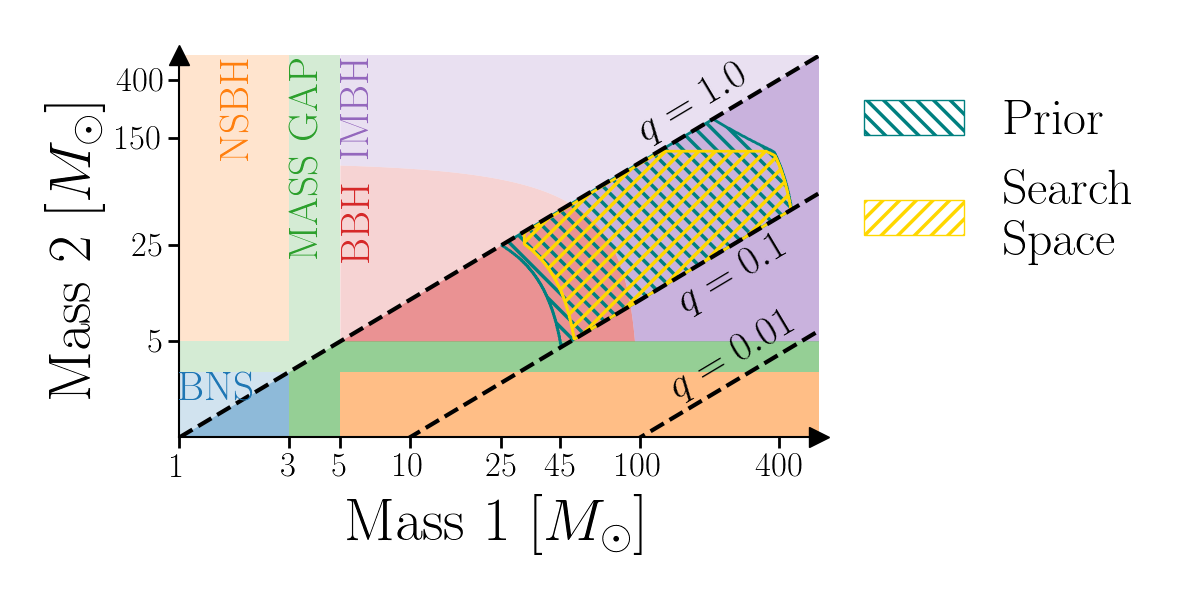
\includegraphics[width=0.75\linewidth]{images/template_bank.png}
}
% time for chunk 14
% 1176955218, Apr 23, 2017, 4:00 UTC
% 1178294418, May 08, 2017, 16:00 UTC
\caption[ BCR search space.]{Component-mass boundaries for our trigger filter and parameter estimation prior. Our search is constrained to the parameter space enclosed by the gold-colored hatches, while our prior is constrained to the slightly larger parameter space enclosed by the teal-colored hatches. The purple region labeled ``IMBH'' is the parameter space where merger remnants may be IMBHs.}\label{fig:templateBank}
\end{figure*}


To evaluate $\{Z^S, Z^G_i, Z^N_i\}$ and calculate the \bcr Eq.~\ref{eq:bcr} for triggers, we carry out Bayesian inference with \bilby~\cite{bilby, bilby_pipe}, employing \dynesty~\cite{dynesty} as our nested sampler. Nested sampling, an algorithm introduced by~\citet{skilling2004, skilling2006}, provides an estimate of the Bayesian evidence and is often utilized for parameter estimation within the LIGO collaboration~\cite{bilby, bilby_paper, pbilby_paper}.

We use a likelihood that marginalizes over coalescence time, the phase at coalescence, and luminosity distance (Eq.~80 from~\citet{intro_to_gw_bayes}). We use identical parameter estimation priors for the glitch and signal models, reflecting our ignorance of the distribution of the population properties of signals and signal-like glitches. The complete list of the priors is in Table~\ref{tab:priors}. 


\begin{table}
    \centering
    \caption{
    Prior settings for the lab-frame parameters used during our parameter estimation. The definitions of the parameters are documented in \citet{bilby_gwtc}~Table~E1. The trigger time $t_c$ is obtained from the data products of \pycbc's O2 search. \label{tab:priors}} 
    \begin{tabular}{c c c c}
    \hline
    Parameter & Shape & Limits \\
    \hline
          $\mathcal{M}/\msun$           & Uniform & 7--180  \\
          $q$                           & Uniform & 0.1--1  \\
          $M/\msun$                     & Constraint & 50--500  \\
          $d_\mathrm{L}/\mathrm{Mpc}$   & Comoving & 100--5000  \\
          $\chi_1$, $\chi_2$            & Uniform & -1--1  \\
          $\theta_{JN}$                 & Sinusoidal & 0--$\pi$  \\
          $\psi$                        & Uniform & 0--$\pi$  \\
          $\phi$                        & Uniform & 0--$2\pi$  \\
          ra                            & Uniform & 0--$2\pi$  \\
          dec                           & Cosine & 0--$2\pi$  \\
          $t_c/\mathrm{s}$              & Uniform & $t_c\pm0.1$  \\
    \hline
    \end{tabular}
\end{table}

The waveform template we utilize is \imrphenomp, a phenomenological waveform template constructed in the frequency domain that models the in-spiral, merger, and ring-down (IMR) of a compact binary coalescence~\citep{khan2016frequency}. Although there exist gravitational-wave templates such as \imrxhm~\cite{imrphenompxhm}, \nrsur~\cite{nrsur7dq4} and \seob~\cite{seobnrv4phm} which incorporate more physics, such as information on higher-order modes, we use \imrphenomp as it is computationally inexpensive compared to others.

To generate the PSD, we take 31 neighboring off-source non-overlapping  4-second  segments of time-series data before the analysis data segment $d_i$. A Tukey window with a 0.2-second roll-off is applied to each data segment to suppress spectral leakage. After this, we fast-Fourier transform and median-average the segments to create a PSD~\cite{ligo_psd}. Like other PSD estimation methods, this method adds statistical uncertainties to the PSD~\cite{psd_student_t, chatziioannou2019noise, Biscoveanu:2020:PhRvD}. To marginalize over the statistical uncertainty, we use the median-likelihood presented by~\citet{psd_student_t} as a post-processing step. We find that this post-processing step improves the search efficiency by $49.26\%$ the details of this calculation are in the Appendix~\ref{sec:psd-marginalization}.

The data we use are the publicly accessible O2 strain data from the Hanford and Livingston detectors, recorded while the detectors are in ``Science Mode''. We obtain the data from the gravitational-wave Open Science Center~\cite{GWOSC} using \gwpy~\cite{gwpy}. 

Finally, with the \candbcr and \bgrdbcr for each time-frame of triggers, we calculate the candidate signal's \pastrobcr. 

\section{\label{sec:Results}Results}

We analyze the O2 candidates with $\totMlab > 55~\msun$ and report candidates with $\pastrobcr\geq0.3$ in Table~\ref{tab:results}. The $\hat{\pi}^S$ and $\hat{\pi}^G$ values utilized for each time-frame are reported in Appendix~\ref{apdx:alphabeta}. 

Various search pipeline \pastro are not mathematically equivalent~\cite{Galaudage:2020:PhRvD}. Moreover, \pastro is not equivalent to \pastrobcr. However, by comparing a candidate's pipeline \pastro with its \pastrobcr, we can compare how significant each pipeline deems the candidate. For comparison, in Table~\ref{tab:results} we report \pastro values from \GWTC~\cite{GWTC1}, PyCBC OGC-2~\cite{pycbc_ogc_2}, PyCBC OGC-3~\cite{pycbc_ogc_2}, PyCBC `single-search'~\cite{pycbc_single_det}, IAS~\cite{IAS1, IAS2}, and \citet{bayesian_odds}'s analyses.

\begin{table*}
\centering
\caption{$\pastrobcr$ table for gravitational wave events and candidates in our search space with $\pastrobcr>0.2$, calculated using Hanford and Livingston observatory data.  Displayed for comparison are significances of events taken from: 
GstLAL \pastroGwtcGstlal~\cite{GWTC1}, 
PyCBC \pastroGwtcPycbc~\cite{GWTC1}, 
IAS \pastroIas~\cite{IAS1, IAS2},  
\pastroPrat~\cite{bayesian_odds}, 
PyCBC `single-search' \pastroSing~\cite{pycbc_single_det}, 
PyCBC OGC-2 \pastroOgcTwo~\cite{pycbc_ogc_2} and
PyCBC OGC-3 \pastroOgcThree~\cite{pycbc_ogc_2}.
The $\tc$ column contains the `GPS' coalescence-times of the gravitational wave events. 
The catalog column displays the first catalog reporting the event on each row (the catalogs labeled IAS-1 and IAS-2 correspond to the candidates published in \citet{IAS1} and \citet{IAS2}).}
\label{tab:results}

\def\arraystretch{1.5} 
\setlength{\tabcolsep}{0.5em}
\begin{NiceTabular}{@{}ll!{\quad}|c|cc!{\quad}c!{\quad}c!{\quad}ccc!{\quad}|c@{}}
\CodeBefore
\rowcolors{2}{white}{gray!10}
\Body


     Event & Catalog & \pastrobcr & \pastroGwtcPycbc & \pastroGwtcGstlal & \pastroIas & \pastroPrat & \pastroSing & \pastroOgcTwo & \pastroOgcThree &          \tc \\
\hline
  GW170104 &  GWTC-1 &        0.97 &              1.00 &               1.00 &             &         1.00 &              &           1.00 &                  & 1167559936.60 \\
  GW170121 &   IAS-1 &        0.83 &                   &                    &        1.00 &         0.53 &              &           1.00 &             1.00 & 1169069154.57 \\
    170209 &       - &        0.32 &                   &                    &             &              &              &                &                  & 1170659643.47 \\
    170222 &       - &        0.58 &                   &                    &             &              &              &                &                  & 1171814476.97 \\
    170302 &   IAS-1 &        0.78 &                   &                    &        0.45 &              &              &                &                  & 1172487817.48 \\
  GW170304 &   IAS-1 &        0.94 &                   &                    &        0.99 &         0.03 &              &           0.70 &             0.70 & 1172680691.36 \\
 GWC170402 &   IAS-2 &        0.60 &                   &                    &        0.68 &         0.00 &              &                &                  & 1175205128.57 \\
  GW170403 &   IAS-1 &        0.54 &                   &                    &        0.56 &         0.27 &              &           0.03 &             0.71 & 1175295989.22 \\
    170421 &       - &        0.27 &                   &                    &             &              &              &                &                  & 1176789158.14 \\
  GW170425 &   IAS-1 &        0.22 &                   &                    &        0.77 &         0.74 &              &           0.21 &             0.41 & 1177134832.18 \\
  GW170608 &  GWTC-1 &        0.99 &              1.00 &               0.92 &             &         1.00 &              &                &                  & 1180922494.50 \\
  GW170727 &   IAS-1 &        0.98 &                   &                    &        0.98 &         0.66 &              &           0.99 &             1.00 & 1185152688.02 \\
  GW170729 &  GWTC-1 &        0.98 &              0.52 &               0.98 &             &         1.00 &              &           1.00 &             0.99 & 1185389807.30 \\
  GW170809 &  GWTC-1 &        0.99 &              1.00 &               0.99 &             &         1.00 &              &           1.00 &             1.00 & 1186302519.75 \\
  GW170814 &  GWTC-1 &        1.00 &              1.00 &               1.00 &             &         1.00 &              &           1.00 &             1.00 & 1186741861.53 \\
 GW170817A &   IAS-2 &        0.92 &                   &                    &        0.86 &         0.02 &              &                &                  & 1186974184.72 \\

\end{NiceTabular}
\end{table*}


\subsection{GWTC-1 Events}
All the confirmed gravitational-wave events from binary black hole mergers reported in \GWTC and within our prior space (specifically GW170104, GW170608, GW170729, GW170809, and GW170814) have $\pastrobcr>0.9$, indicating a high probability of an astrophysical signal. 

In addition to the above confirmed gravitational-wave events from \GWTC, we have also analyzed several candidate events from \GWTC, most of which have low \pastrobcr. For example, consider the candidate event 170412 ($\tc = 1176047817$), assigned a $\pastro$ of $0.06$ by \gstlal and has a $\pastrobcr$ of $0.01$. This candidate was reported to be excess power caused due to noise appearing non-stationary between 60-200 Hz~\cite{GWTC1}. This candidate acts as an example of how $\pastrobcr$ may be utilized to eliminate candidates originating from terrestrial noise sources. 

\subsection{IAS Events}
Our analysis of the IAS events and candidates with $\totMlab\gtrsim55~\msun$ in O2 has resulted in one event with disfavored $\pastrobcr<0.5$ (GW170425), and five events and two candidates with $\pastrobcr\geq0.5$ (GW170121, GW170304, 170302, GWC170402, GW170403, GW170727, GW170817A). From this list, four events (GW170121, GW170304, GW170727, GW170817A) have $\pastrobcr>0.8$ and $\pastro>0.9$ reported from other pipelines, making them viable gravitational-wave event candidates.  

GWC170402, detected by \citet{IAS2}, is reported to originate from a binary with non-zero eccentricity~\cite{IAS2}. As we used a non-eccentric waveform during analysis, we may be under estimating this event's significance at $\pastrobcr\leq0.6$. Finally, GW170425 which has $\pastrobcr<0.25$ also has low \pastro reported in OGC-2 and OGC-3 \cite{pycbc_ogc_2,pycbc_ogc_3}, suggesting that GW170425 may have been false alarm.


\subsection{New Candidate Events}
Although no IMBH detections are made with the \bcr, a marginal stellar mass black hole merger candidate 170222 has been discovered with a $\pastrobcr\sim0.6$. This candidate has a SNR$\sim7.7$, low spin magnitudes, and source-frame component masses of $({47.16}_{-5.77}^{+8.00}, {35.50}_{-6.35}^{+5.79}) \msun$ ($90\%$ credible intervals), making it one of the heavier black-hole mergers from O2 and \GWTC. This candidate may be of interest as one component black hole may lie in the pair-instability mass gap ($55^{+10}_{-10}-148^{+13}_{-12}\msun$)~\cite{Woosley:2021:arXiv, Heger:2002:ApJ}. More details on the candidate are presented in Appendix~\ref{apdx:170222}. The remaining coherent trigger candidates all have $\pastrobcr<0.5$, making them unlikely to originate from astrophysical sources. 

\section{\label{sec:Conclusion}Conclusion}

In this paper, we demonstrate that the Bayesian Coherence Odds-Ratio \bcr~\cite{BCR1} can be used as a ranking statistic to provide a measure of significance for gravitational-wave signals originating from CBCs with total masses between $55~\msun$ and $400~\msun$, a range that includes IMBHs. To compute the \bcr for candidates, we utilize Bayesian inference to explicitly calculate the probability of data under various hypotheses (the hypotheses that the data contains a coherent signal, just noise, or an incoherent glitch). This Bayesian ranking method takes a step towards building a unified Bayesian framework that provides a measure of significance for candidates and estimates their parameters, utilizing the same level of physical information incorporated during detected parameter estimation studies. 

In our study, we analyze O2 binary-black hole events and candidates with $\totMlab > 55~\msun$ reported by the \pycbc search~\cite{pycbc_ogc_2}, the \IAS-team~\cite{IAS1, IAS2} and those reported in \GWTC~\cite{GWTC1}. Using \pastrobcr, we find that the \GWTC events have high probabilities of originating from an astrophysical source. We also find that some of the \GWTC marginal triggers that have corroborated terrestrial sources (for example, candidate 170412) have low \pastrobcr, indicating this method's ability to discriminate between terrestrial artifacts and astrophysical signals. Our analysis of the \IAS events demonstrates that GW170121, GW170304, GW170727, and GW170817A are likely to originate from astrophysical sources ($\pastrobcr\geq0.8$), while GW170425 is not ($\pastrobcr<0.25$). Finally, we do not identify any new gravitational-wave events, but we find a new marginal binary-black hole merger candidate, 170222. 

Although our analysis targets triggers with $\totMlab \gtrsim 55~\msun$, this method can be extended to include the entire range of LIGO-detectable gravitational-wave sources. Additionally, to further improve the method's infrastructure, we can use more robust gravitational-wave templates (such as templates that incorporate higher-order modes and orbital precession) and sophisticated glitch models. Future analysis can also incorporate data from all available detectors in a network to increase the sensitivity of \pastrobcr. 


%%%%%%---ACKNOWLEDGMENTS---%%%%%%%%%%%%
\begin{acknowledgments}
The authors gratefully thank the \pycbc team for providing the gravitational-wave foreground, background, and simulated triggers from \pycbc's search of O2's data. We also warmly thank Ian Harry and Thomas Dent for answering questions about the \pycbc search's data products.  

We gratefully acknowledge the computational resources provided by the LIGO Laboratory—Caltech Computing Cluster and supported by NSF grants PHY-0757058 and PHY-0823459, and thank Stuart Anderson for his assistance in resource scheduling.

All analyses (inclusive of test and failed analyses) performed for this study used $~1.3\mathrm{M}$ core-hours, amounting to a carbon footprint of $~167\ \mathrm{t}$ of CO$_2$ (using the U.S. average electricity source emissions of $0.429\ \text{kg/kWh}$~\cite{greenhouse} and $0.3\ \text{kWh}$ for each CPU).

This work is supported by the Australian Research Council (ARC) Centre of Excellence CE170100004. This material is based upon work supported by NSF’s LIGO Laboratory, a major facility fully funded by the National Science Foundation. This research has used data, software, and web tools obtained from the Gravitational Wave Open Science Center (https://www.gw-openscience.org), a service of LIGO Laboratory, the LIGO Scientific Collaboration, and the Virgo Collaboration. The U.S. National Science Foundation funds LIGO. Virgo is funded by the French Centre National de Recherche Scientifique (CNRS), the Italian Istituto Nazionale della Fisica Nucleare (INFN), and the Dutch Nikhef, with contributions by Polish and Hungarian institutes.

\end{acknowledgments}
%%%%%%%%%%%%%%%%%%%%%%%%

\appendix



\section{Bayesian Evidence Evaluation}\label{sec:bayesianEvidEval}

\subsection{Noise Model}
We assume that each detector's noise is Gaussian and stationary over the period being analyzed~\cite{ligo_psd}. In practice, we assume that the noise has a mean of zero that the noise variance $\sigma^2$ is proportional to the noise power spectral density (PSD) \psd of the data. Using the \psd, for each frequency-domain data segment $d_i$ in each of the $i$ detectors in a network of $D$ detectors, we can write 
\begin{equation}
\label{eq:zn}
Z^N_i = \mathcal{N}(d_i|\mu=0,\sigma^2=\psd),
\end{equation}
where $\mathcal{N}$ is a normal distribution. 

\subsection{Coherent Signal Model}
We model coherent signals using a binary black hole waveform template \template, where the vector \parameters contains a point in the 12-dimensional space describing aligned-spin binary-black hole mergers. For the signal to be coherent, \parameters must be consistent in each 4-second data segment $d_i$ for a network of $D$ detectors. Hence, the coherent signal evidence is calculated as
\begin{equation}
\label{eq:zs}
Z^S = \int\limits_{\parameters} \prod\limits^{D}_{i=1} \left[ \mathcal{L}(d_i|\template)\right] \pi(\parameters | \mathcal{H}_S)\  \text{d}\parameters \ ,
\end{equation}
where $\pi(\parameters| \mathcal{H}_S)$ is the prior for the parameters in the coherent signal hypothesis $\mathcal{H}_S$, and $\mathcal{L}(d_i|\template)$ is the likelihood for the coherent signal hypothesis that depends on the gravitational-wave template \template and its parameters \parameters. 

\subsection{Incoherent Glitch Model}
Finally, as glitches are challenging to model and poorly understood, we follow \citet{bci} and utilize a surrogate model for glitches. The glitches are modeled using gravitational-wave templates  \template with uncorrelated parameters amongst the different detectors such that  $\parameters_i \neq \parameters_j$ for two detectors $i$ and $j$~\cite{bci}.  Modeling glitches with \template captures the worst-case scenario: when glitches are identical to gravitational-wave signals (excluding coherent signals). Thus, we can write $Z^G_i$ as 
\begin{equation}
\label{eq:zg}
Z^G_i = \int\limits_{\parameters} \mathcal{L}(d_i|\template)\ \pi(\parameters| \mathcal{H}_G)\  \text{d}\parameters  \ ,
\end{equation}
where $\pi(\theta| \mathcal{H}_G)$ is the prior for the parameters in the incoherent glitch hypothesis $\mathcal{H}_G$. 



\section{Tuning the prior-odds}\label{apdx:tuning-prior-odds}

After calculating the \bcr for a set of background triggers and simulated triggers from as stretch of detector-data (a data chunk), we can compute probability distributions for the background and simulated triggers, $p_b(\bcr)$ and $p_s(\bcr)$. We expect the background trigger and simulated signal \bcr values to favor the incoherent glitch and the coherent signal hypothesis, respectively. Ideally, these distributions representing two unique populations should be distinctly separate and have no overlap in their \bcr values. The prior odds parameters $\hat{\pi}^S$ and $\hat{\pi}^G$ from Eq.~\ref{eq:bcr} help separate the two distributions. Altering $\hat{\pi}^S$ translates the \bcr probability distributions while adjusting $\hat{\pi}^G$ spreads the distributions (refer to Appendix A of \citet{BCR1}). Although Bayesian hyper-parameter estimation can determine the optimal values for $\hat{\pi}^S$ and $\hat{\pi}^G$, an easier approach is to adjust the parameters for each data chunk's \bcr distribution. In this study, we tune $\hat{\pi}^S$ and $\hat{\pi}^G$ to maximally separate the \bcr distributions for the background and simulated triggers. 

To calculate the separation between $p_b(\bcr)$ and $p_s(\bcr)$, we use the Kullback--Leibler divergence (KL divergence) $D_{KL}$, given by
\begin{equation}
    D_{KL}(p_b | p_s) = \sum\limits_{x\in \bcr} p_b(x) \log \left( \frac{p_b(x)}{p_a(x)} \right)  \ .
\end{equation}
The $D_{K.L.}=0$ when the distributions are identical and increases as the asymmetry between the distributions increases. 

We limit our search for the maximum KL-divergence in the $\hat{\pi}^S$ and $\hat{\pi}^G$ ranges of $[10^{-10}, 10^0]$. We set our values for $\hat{\pi}^S$ and $\hat{\pi}^G$ to those which provide the highest KL-divergence and calculate the \bcr for candidate events present in this data chunk. Note that we conduct the analysis in data chunks of a few days rather than an entire data set of a few months as the background may be different at different points of the entire data set.






\section{Marginalizing over PSD statistical uncertainties}\label{sec:psd-marginalization}
To generate the results presented in Table~\ref{tab:results}, we applied a post-processing step to marginalize the uncertainty in the PSD. In Fig.~\ref{fig:bcrCdf}, we demonstrate the impact of the post-processing step. Marginalizing over uncertainty in the PSD yields an improvement in the separation of the noise and signal distributions (left plot). Quantitatively, at a threshold $\bcr^T=0$ the post-processing step results in a reduction in the number of background $\bcr > \bcr^T$ from $60.7\%$ to $25.28\%$ in the August 13 - 21, 2017 time-frame of data. For the entirety of O2, PSD marginalization resulted in a $49.26\%$ improvement in search efficiency. 


\begin{figure*}
    \centering
    \begin{subfigure}
        \centering
        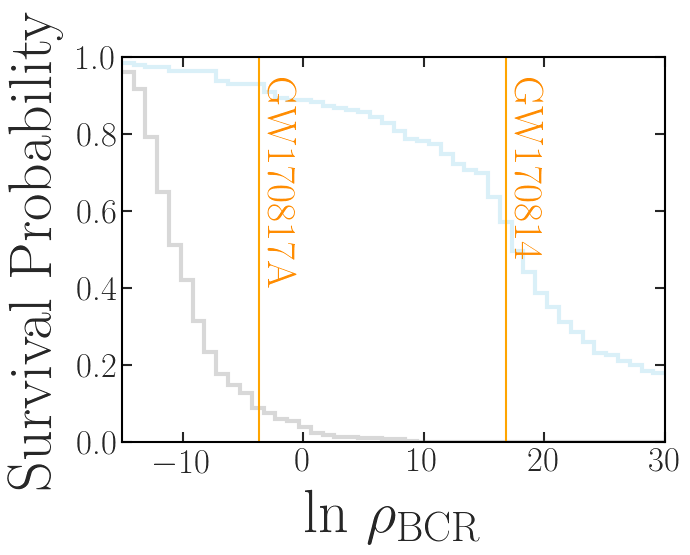
\includegraphics[width=0.45\linewidth]{reweighted_bcr_cdf_smaller_legend.png}
    \end{subfigure}
    ~ 
    \begin{subfigure}
        \centering
        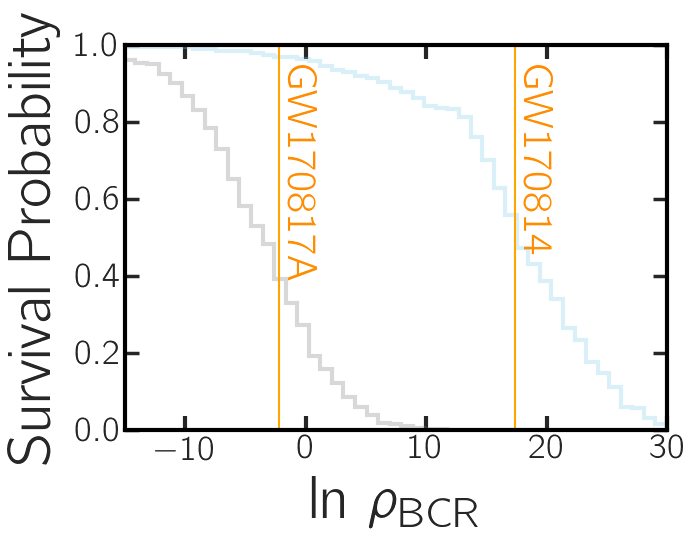
\includegraphics[width=0.45\linewidth]{orig_bcr_cdf_smaller_legend.png}
    \end{subfigure}
    \caption{
    Histograms represent the survival function (1-CDF) from our selection of background triggers (gray) and simulated signals (blue) triggers obtained from \pycbc's search of data from $\text{August 13 - 21, 2017}$. Vertical lines mark the $\text{ln}\ \bcr$ of \IAS's GW170817A and \GWTC's GW170814.
    Left: Survival functions using the post-processing step to marginalize over PSD statistical uncertainties. Right: Survival functions without the post-processing step. Without the post-processing step, there is a greater overlap between the background (gray) and foreground (blue) survival functions.
    \label{fig:bcrCdf}}
\end{figure*}






\section{Tuned prior odds}\label{apdx:alphabeta}

O2 lasted several months, over which the detector's sensitivity varied. Hence, a part of our analysis entailed tuning the prior odds for obtaining a signal and a glitch, $\hat{\pi}^S$ and $\hat{\pi}^G$, as described in Section~\ref{sec:method}. Table~\ref{tab:priorodds} presents the signal and glitch prior odds utilized for each time-frame of O2 data. 
\begin{table}
\centering
\caption{The prior odds used for each time-frame of data from O2. Each time frame commences at the start date and concludes at the following time-frame's start date.
    }
\label{tab:priorodds}
\def\arraystretch{1.5} 
\setlength{\tabcolsep}{0.5em}
\begin{tabular}{c|cc}

 Start Date &    $\hat{\pi}^S$ &    $\hat{\pi}^G$ \\
\midrule
 2016-11-15 &        - &        - \\
 2016-11-30 &        - &        - \\
 2016-12-23 & 1.00E+00 & 6.25E-01 \\
 2017-01-22 & 1.00E+00 & 2.33E-02 \\
 2017-02-03 & 1.00E-10 & 2.44E-01 \\
 2017-02-12 & 1.76E-08 & 5.96E-02 \\
 2017-02-20 & 6.55E-10 & 2.22E-03 \\
 2017-02-28 & 1.00E-10 & 5.96E-02 \\
 2017-03-10 & 2.56E-10 & 3.91E-01 \\
 2017-03-18 & 1.60E-10 & 1.00E+00 \\
 2017-03-27 & 1.10E-08 & 5.96E-02 \\
 2017-04-04 & 3.73E-02 & 2.33E-02 \\
 2017-04-14 & 1.05E-09 & 2.44E-01 \\
 2017-04-23 & 2.68E-09 & 1.46E-02 \\
 2017-05-08 & 1.00E+00 & 2.44E-01 \\
 2017-06-18 & 6.55E-10 & 3.39E-04 \\
 2017-06-30 & 2.02E-05 & 5.69E-03 \\
 2017-07-15 & 1.05E-09 & 9.54E-02 \\
 2017-07-27 & 1.00E+00 & 2.12E-04 \\
 2017-08-05 & 2.12E-04 & 3.73E-02 \\
 2017-08-13 & 2.68E-09 & 8.69E-04 \\
 2017-08-21 &        - &        - \\

\end{tabular}
\end{table}


Tuning the prior odds can dramatically affect the \pastrobcr. For example, consider Table~\ref{tab:tuningresults}, which reports tuned \pastrobcr and un-tuned \untunedpastrobcr (where $\hat{\pi}^S=1$ and $\hat{\pi}^G=1$) for various events and candidates. By tuning the prior odds, the \pastrobcr for some IAS events (for example, GW170403 and GW170817A) can change by more than 0.5, resulting in the promotion/demotion of a candidate's significance.


\begin{table}
\centering
\caption{The BCR p-astro after tuning the prior odds, \pastrobcr, and without tuning the prior odds, \untunedpastrobcr (where $P^S=1$ and $P^G=1$).}
\label{tab:tuningresults}
\def\arraystretch{1.5} 
 \setlength{\tabcolsep}{0.5em}
\begin{tabular}{ll|c c}

     Event &  Catalog & \pastrobcr & \untunedpastrobcr \\
\hline
    161202 &  - &        0.09 &               0.41 \\
  GW170104 &   GWTC-1 &        0.94 &               0.93 \\
  GW170121 &    IAS-1 &        0.76 &               0.72 \\
    170206 &  - &        0.11 &               0.52 \\
    170222 &  - &        0.49 &               0.49 \\
    170302 &    IAS-1 &        0.64 &               0.54 \\
  GW170304 &    IAS-1 &        0.83 &               0.81 \\
 GWC170402 &    IAS-2 &        0.38 &               0.01 \\
  GW170403 &    IAS-1 &        0.33 &               0.89 \\
  GW170425 &    IAS-1 &        0.10 &               0.22 \\
  GW170608 &   GWTC-1 &        0.95 &               0.95 \\
  GW170727 &    IAS-1 &        0.92 &               0.96 \\
  GW170729 &   GWTC-1 &        0.96 &               0.94 \\
  GW170809 &   GWTC-1 &        0.98 &               0.99 \\
  GW170814 &   GWTC-1 &        1.00 &               1.00 \\
 GW170817A &    IAS-2 &        0.83 &               0.36 \\

\end{tabular}
\end{table}



\section{A closer look at 170222}\label{apdx:170222}
PyCBC found the candidate 170222 with $\mathcal{M}_c=49.46$ and $q=0.68$, values contained inside the $90\%$ credible intervals of our posterior probability distributions for 170222. Some of the posteriors produced as a by-product of our \bcr calculation can be viewed in Fig.~\ref{fig:170222}.

\begin{figure*}
    \centering
    \begin{subfigure}
        \centering
        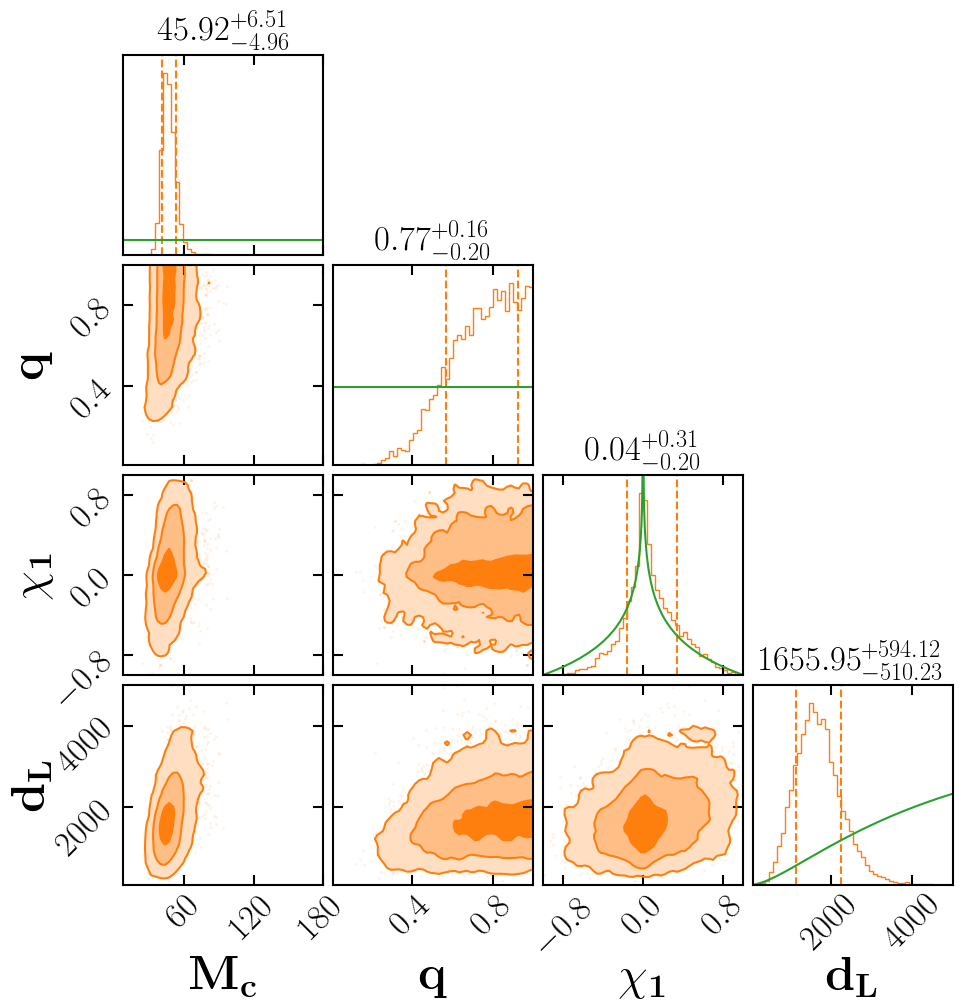
\includegraphics[width=0.45\linewidth]{170222_prior_posterior.png}
    \end{subfigure}
    ~ 
    \begin{subfigure}
        \centering
        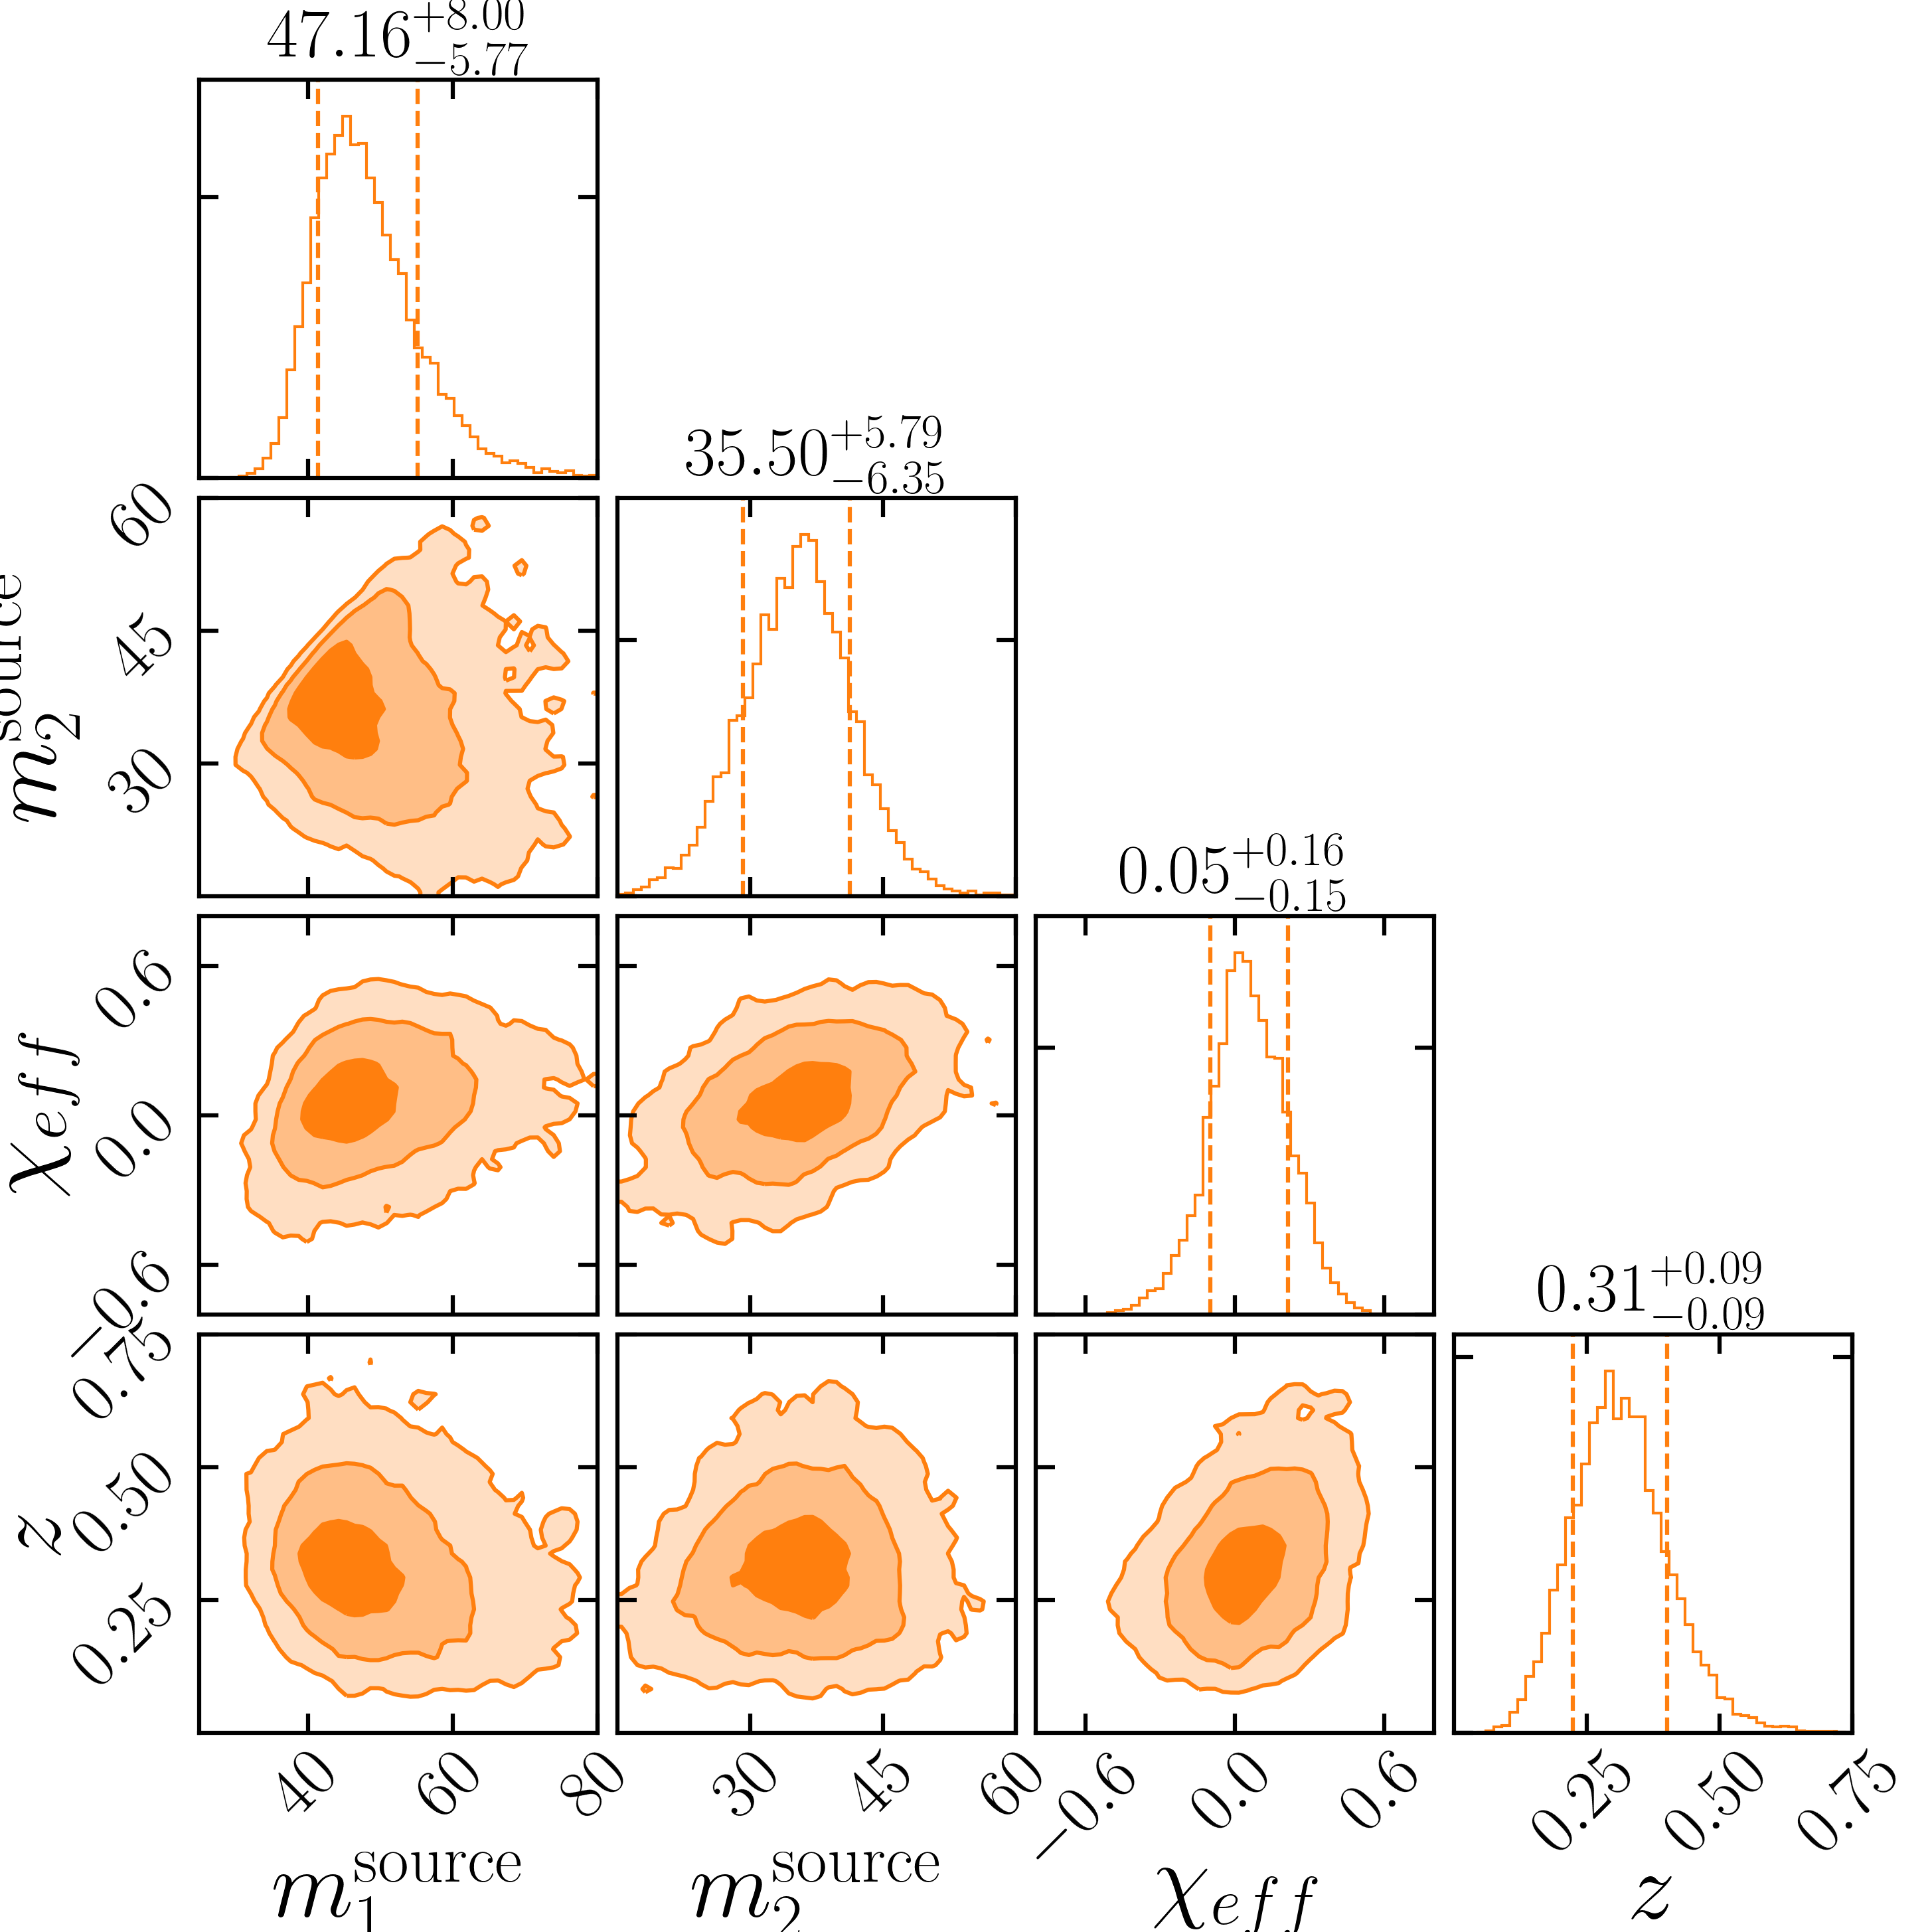
\includegraphics[width=0.45\linewidth]{170222_source_posterior.png}
    \end{subfigure}
    \caption{Posterior distributions for 8 parameters of 170222. 
    Left: Posterior probability distributions for 4 of the 12 search parameters.
    Right: Posterior probability distributions for 4 derived parameters.
    \label{fig:170222}}
\end{figure*}





\bibliography{high_mass_bib}

\end{document}


